\documentclass[10pt,notitlepage]{article}
\usepackage{graphicx}
\usepackage{verbatim}
\usepackage[portuguese]{babel}
\usepackage[utf8]{inputenc}
\usepackage[hmargin=2cm,vmargin=3.5cm,bmargin=2cm]{geometry}

\begin{document}

%%%CAPA%%%
\begin{titlepage}

\begin{center}


\begin{figure}
\centering

\includegraphics[scale=0.5]{logo.pdf}
\end{figure}





Escola de Engenharia \\  Departamento de Informática \\ Licenciatura em Engenharia Informática \\~\\~  \\~ \\~ \\~ \\~ \\~ \\~ \\




{\Huge Serviço de Contagem}
\\~ \\~ \\~ \\
Sistemas Operativos
  \vfill





\vspace{1.5cm}
 \begin{flushleft}  Autores: \\
 \textbf{Bruno Pereira\hspace{35pt} Número:69303\\João Rua \hspace{55pt}   Número:41841\\João Mano \hspace{48pt}           Número:69854\\}
 %%\date{Abril 2014}%%
\end{flushleft}

 \vspace{0.8cm}
 Data Junho 2014
\end{center}

\end{titlepage}




\tableofcontents

\newpage

\section{Objectivos}
~\\
Este documento apresenta o nosso projecto no âmbito da unidade curricular de Sistemas Operativos da Licenciatura de Engenharia Informática.\\
O objectivo do trabalho consiste na implementação, em linguagem C, de um serviço de contagem. Este deverá permitir registar persistentemente incrementos em contadores,bem como reportar valores de contadores, individuais ou agregados. Cada contador tem um nome hierárquico, constituído por uma sequência de strings.

~\\
\section{Estrutura da aplicação}
~\\
Os clientes comunicam com o servidor através da api(contagem) usando para isso os seguintes comandos:
\begin{itemize}
\item incrementar
\item agregar
\end{itemize}

A api utiliza um parser que separa os parâmetros da operação introduzida, para o mais fácil
processamento da mesma.\\
Os parâmetros são transmitidos depois através de um named pipe para servidor.


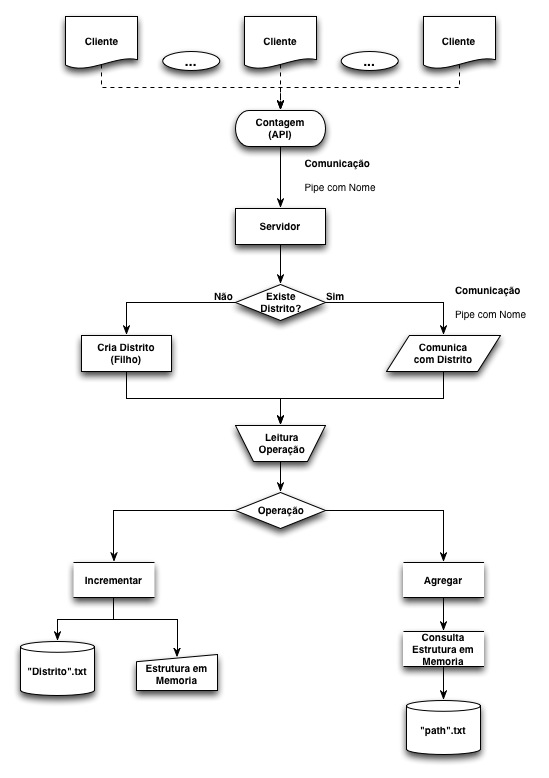
\includegraphics[width=0.90\textwidth]{so.jpg}


\subsection{Servidor}
~\\
O servidor verifica a existência de um processo filho, responsável pela distrito, consultando a estrutura de filhos existente.\\
Caso não exista ainda um filho responsável pelo distrito introduzido, ele ira criar o respectivo filho que ficara responsável pelos dados desse distrito.
~\\~\\
O servidor poderá responder as seguintes operações:
\begin{itemize}
\item Incrementar- Envia para o processo filho responsável pelo distrito o respectivo comando.
\item Agregar- Envia para o processo filho responsável pelo distrito o respectivo comando.
\item Lista [distrito]- Envia para o processo filho responsável pelo distrito o respectivo comando, acaso não seja introduzido o distrito, envia para todos os processos filhos o comando lista
\item Filhos- Mostra a estrutura “Filhos” onde estão guardados todos os processos filhos criados pelo servidor para gerir os respectivos distritos.
\end{itemize}
~\\~\\
Toda a comunicação existente entre o servidor e o processo filho é efectuada através de um named pipe, com o nome desse distrito.
Os filhos ficam a espera de operações, que serão transmitidas pelo servidor.
Aquando da recepção dessa operação, será verificada qual a procedimento a ser realizado, entre as seguintes opções:
\begin{itemize}
\item Incrementar- Processo através do qual é incrementado um contador na estrutura de dados e guardado no ficheiro respectivo a esse filho.
\item Agregar- Processo através do qual é agrupada um conjunto de informações conforme os parâmetro introduzidos pelo cliente.
\item Listar- Apresenta a estrutura actual do distrito.
\end{itemize}



\newpage
\subsubsection{Estrutura do Servidor}



\begin{figure}[h]
\centering
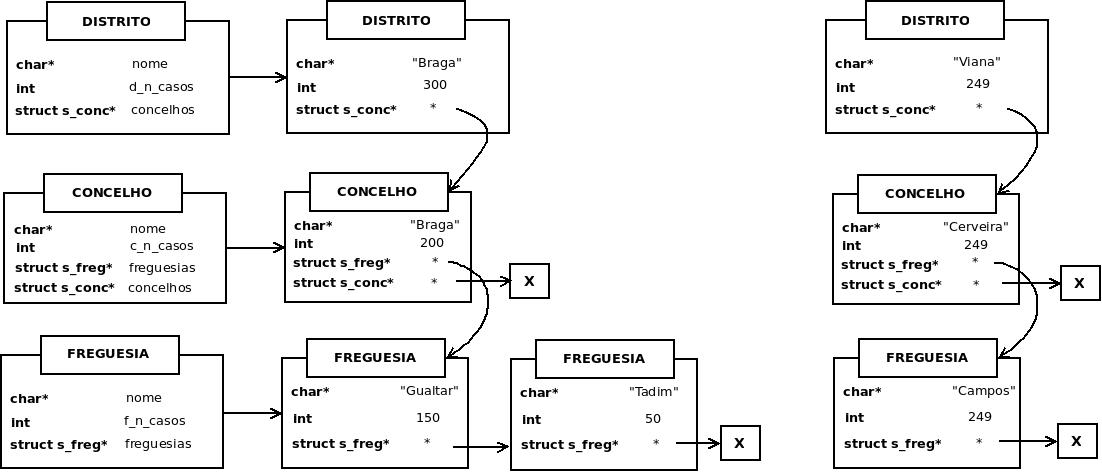
\includegraphics[scale=0.45]{StructsDistConcFreg.jpeg}
\caption{Estrutura geral}
\end{figure}



\begin{figure}[h]
\centering
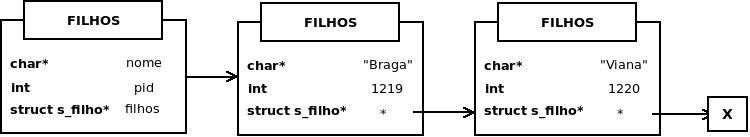
\includegraphics[scale=0.45]{StructsFilhos.jpeg}
\caption{Estrutura dos filhos}
\end{figure}



\section{Testes Efectuados}

Foram realizados testes exaustivos com múltiplos clientes, activos simultaneamente, cada um com milhares de pedidos, de forma a comprovar a robustez e performance da nossa aplicação.\\
Todos os testes realizados e seus respectivos resultados encontram-se na mesma pasta deste relatório.











\section{Conclusão}
Com a chegada do fim deste relatório chegou a altura de se tecerem as conclusões finais.
A implementação deste serviço de contagem fez-nos entender um pouco mais sobre a forma como são criados e mobilizados os processos dentro do sistema operativo. A interpretação de sequências de comandos em pipelines permitiu-nos perceber como é feita a sua execução sequencial numa única
pipeline, assim como o multi processamento de instruções(execução de vários comandos em diferentes pipelines).\\
Consideramos que a nossa solução satisfaz todos os requisitos exigidos pelo enunciado.
Em suma, consideramos que este trabalho foi uma mais-valia no sentido em que nos permitiu
aplicar grande parte da matéria abrangida pela unidade curricular.






 
\end{document} 